\documentclass[a4paper, 11pt]{scrreprt}
\usepackage[utf8]{inputenc}
\usepackage[ngerman]{babel}
\usepackage[T1]{fontenc}
\usepackage{lmodern}
\usepackage{amsmath,amssymb,amstext,amsfonts,mathrsfs, amsthm}
\usepackage{graphicx}
\usepackage{color}

\usepackage{marginnote}

\pagestyle{headings}

\newtheorem{defi}{Definition}[section]
\newtheorem{prop}[defi]{Proposition}
\newtheorem{theorem}[defi]{Theorem}
\newtheorem{coro}[defi]{Corollary}
\newtheorem{lemma}[defi]{Lemma}

\newcommand{\RR}{\mathbb{R}}
\newcommand{\EE}{\mathbb{E}}
\newcommand{\ZZ}{\mathbb{Z}}
\newcommand{\NN}{\mathbb{N}}
\newcommand{\FF}{\mathcal{F}}

\newcommand{\student}[1]{\marginnote{{\normalfont\bf #1}}}

\title{Abschlussarbeit Fallstudien der math. Modellbildung}
\author{Manuela Lambacher, Dominik Otto, Andreas Wiedemann}
\date{\today}

\begin{document}
\parindent 0pt
\maketitle
\tableofcontents


\chapter{Das Marchenko-Pastur-Gesetz}

\section{Das Marchenko-Pastur-Gesetz}

Sei \(Y_N\) eine \(N\times M(N)\)-Matrix mit unabhängigen zentrierten Einträgen mit Varianz \(1\),
	\[\sup_{j,k,N} \EE\left[ | Y_N(j,k)|^q\right] = C_q < \infty \qquad \forall q \in \NN\]
und \(M(N) \in \NN\) so, dass
	\[\lim_{N\to\infty} \frac{M(N)}{N} = \alpha \in[1,\infty). \]
Sei weiterhin die Wishart-Matrix gegeben als 
	\[W_N = \frac{1}{N}Y_NY_N^T,\]
und habe die empirische Eigenwertverteilung
	\[L_N = \frac{1}{N} \sum_{j=1}^{N} \delta_{\lambda_j} \]
und das Zustandsdichtemaß \(\overline{L_N} = \EE[L_N]\). Dann gilt die Konvergenz
	\[\overline{L_N} \xrightarrow{\text{w}} f_{\alpha}(x)dx \quad(N\to\infty)\]
im Raum der Wahrscheinlichkeitsmaße auf \(\RR\), wobei
	\[f_{\alpha}(x)=\frac{1}{2\pi x}\sqrt{(x-(1-\sqrt{\alpha})^2_{+}((1+\sqrt{\alpha})^2_{+}} \]

\newpage
\section{Beweis des Marcenko-Pastur Gesetzes}
Zuerst bringen wir \(N^{l+1} \langle \overline{L_N}, x^l \rangle\) in eine Form, die eine weitergehende Untersuchung ermöglicht:
\begin{equation}
\begin{split}
		N^{l+1} &\langle \overline{L_N}, x^l \rangle\ 
		= N^{l+1} \cdot \int x^l \overline{L_N}(dx) 
		= N^{l+1} \cdot \frac{1}{N} \cdot \EE[tr(W^l_N)] 
		= N^l \sum_{j_1,...,j_l = 1}^N \EE\left[\prod_{p = 1}^l W_{j_p,j_{p+1}}\right] \\
		&= N^l \sum_{j_1,...,j_l = 1}^N \EE\left[\prod_{p = 1}^l \frac{1}{N} \sum_{k = 1}^{M(N)} Y_N(j_p,k) \cdot Y_N(j_{p+1},k) \right] \\
		&= \sum_{j_1,...,j_l = 1}^N \EE \left[\left(\sum_{k = 1}^{M(N)} Y_N(j_1,k) \cdot Y_N(j_2,k)\right) \cdot \left(\prod_{p = 2}^l \sum_{k = 1}^{M(N)} Y_N(j_p,k) \cdot Y_N(j_{p+1},k) \right) \right] \\
		&= \sum_{j_1,...,j_l = 1}^N \EE\left[	\prod_{p = 2}^l \sum_{k_1,k_2 = 1}^{M(N)} Y_N(j_1,k_1) \cdot Y_N(j_2,k_1) \cdot Y_N(j_p,k_2) \cdot Y_N(j_{p+1},k_2) \right] \\
		&= ... \\
		&= \sum_{j_1,...,j_l = 1}^N \sum_{k_1,...,k_l = 1}^{M(N)} \EE[Y_N(j_1,k_1) Y_N(j_2,k_1) Y_N(j_2,k_2) Y_N(j_3,k_2) ... Y_N(j_l,k_l) Y_N(j_1,k_l)]\\
 &= \sum_{r_1,r_2 = 1}^l \sum_{\substack{J:v(J)=s_1\\ K:v(K)=s_2 }} \EE[Y_N(J,K)]
\end{split}
\end{equation}
wobei 
\begin{align*}
	&J=(j_1,j_2,j_2,...,j_l,j_l,j_1), K=(k_1,k_1,...,k_l,k_l),\\
	&v: \NN^{2l}\to \NN,\ v(X) := \text{Anzahl der verschiedenen Indizes in X}
\end{align*}
Die einzelnen Summanden können also als Eulergraphen auf \(s_1+s_2 \)Knoten und \(2l\) Kanten interpretiert werden.
Damit ergeben sich die drei Fälle (setze \(s = s_1+s_2\) )
\begin{itemize}
	\item \(s < l+ 1\)\\
		\begin{equation}
			\begin{split}
			\EE[Y_N(J,k)] &\leq \prod_{n=1}^l \left(\sup_{j,k,N}\EE\left[|Y_N(j,k)|^l\right]\right)^{\frac 1 l} \\
			& = \prod_{n=1}^l C_l^{\frac 1 l} = C_l
			\end{split}
			\end{equation}
	Außerdem gilt: 
		\begin{align}
			\#\{J: v(J)=s_1\} &\leq \begin{pmatrix} N \\ s_1 \end{pmatrix} s_1^l \leq N^{s_1}s_1^l \\
			\#\{K: v(K)=s_2\} &\leq \begin{pmatrix} M(N) \\ s_2 \end{pmatrix} s_2^l \leq M(N)^{s_2}s_2^l
		\end{align}
	Somit ergibt sich aus \((2.2) - (2.4)\): 
	\begin{equation}
		\frac {1}{N^{l+1}} \sum_{\substack{J:v(J)=s_1\\ K:v(K)=s_2 }} \EE[Y_N(J,K)] < C_l (l+1)^l \frac{N^{s_1} M(N)^{s_2}}{N^{l+1}} \xrightarrow{N\to\infty} 0
	\end{equation}
		
	\item \(s> l+1\) \\
		Nach Lemma aus der Vorlesung exisitert eine einfache, echte Kante und somit \(\EE[Y_N(J,K)]=0\), da die Matrixeinträge unabhängig sind.
	\item \(s=l+1\)\\
		Es tragen also nur die Graphen auf \(l+1\) verschiedenen Knoten zu \(\lim_{N\to\infty} \langle \overline{L_N}, x^l \rangle \) bei. Diese Graphen haben die Struktur eines Doppelbaumes%, denen man geordnete, nicht überkreuzende Paarzerlegungen und damit auch Catalanpfade zuordnen kann.
\end{itemize}
%\textbf{Weitere Analyse von \(\beta_l\):}\\
Diese Doppelbaumstruktur lässt sich wie folgt nutzen:\\
Wähle für einen Doppelbaum \(r\) Knoten aus den \(k\)-Knoten und \(l+1-r\) Knoten aus den \(j\)-Knoten. Dann folgt:
\begin{equation}
	\begin{split}
	\sum_{J,K: v(J)+v(K) = l+1} \EE[Y_N(J,K)] = &\sum_{r=1}^{l}\begin{pmatrix} N\\ l+1-r\end{pmatrix} (l+1-r)! \begin{pmatrix} M(N)\\r\end{pmatrix} r! \\
	&\cdot \#\{\text{Doppelbäume mit }l+1-r\ j\text{-Knoten und } r\ k\text{-Knoten}\} \\
	%=& \sum_{r=1}^{l} \begin{pmatrix} N\\ l+1-r\end{pmatrix} (l+1-r)! \begin{pmatrix} M(N)\\r\end{pmatrix} r! \cdot \begin{pmatrix} 2l-2\\2r-2\end{pmatrix} C_{l-r}
	\end{split}
\end{equation}
%Eine Formel für die Anzahl der Doppelbäume folgt aus der nachfolgenden Konstruktion (Anm: das -2 folgt immer, da die beiden Wurzelkanten fest 0 im Catalanpfad sind; Die Catalanzahl für l-r, weil von dem gesamten Pfad der Länge 2l 2r Stücke flach sind und die übrigen wie beim normalen Catalanpfad aufgeteilt werden können) \\ \\
Ein Doppelbaum mit \(r\  k\)-Knoten und \((l+1-r)\ j\)-Knoten kann wie folgt als Catalan-Pfad der Länge \(l\) interpretiert werden:\\
Wähle als Wurzel des Baumes einen \(j\)-Knoten und gliedere den Baum in Ebenen, wobei die Wurzel in der 0.Ebene liegt.(Die \(k\)-Knoten liegen also in ungeraden Ebenen, die \(j\)-Knoten in geradenen Ebenen) Verweise jede Kante mit einer Richtung, sodass bei jeder Doppelkante eine Kante von dem Knoten wegführt und eine zu ihm hinführt. Durchlaufe den Baum mit Hilfe der Tiefensuche und nummeriere die Kanten in der Reihenfolge, wie sie bei der Tiefensuche durchlaufen werden. Konstruiere den Catalan-Pfad wie folgt:\\
\begin{itemize}
	\item Wird ein Knoten zum ersten Mal erreicht: \((+1)\)
	\item Kehrt man zu einem bereits besuchten Knoten zurück :\((-1)\)
	
\end{itemize}
Da der Baum durch Tiefensuche durchlaufen wird, gibt die Entfernung eines Knotens zur Wurzel die Anzahl der nötigen Schritte wieder, die benötigt werden, um ihn zum ersten Mal zu erreichen. Da die \(j\)-Knoten in den geraden Ebenen und die \(k\)-Knoten in den ungeraden Ebenen liegen, ergibt sich, dass sich die \(j\)-Knoten stets auf den geraden Niveaus und die \(k\)-Knoten stets auf den ungeraden Niveaus des Catalan-Pfades befinden. 


%\begin{itemize}
%	\item Alle Kanten zwischen der Wurzel und der ersten Ebene sind Flachstücke: \((+0)\)
%	\item Wenn eine Kante von ungerader Ebene aufwärts auf gerade Ebene führt: \((+1)\)
%	\item Wenn eine Kante von gerader Ebene abwärts auf ungerade Ebene führt: \((-1)\)
%	\item Die restlichen Kanten sind alle Flachstücke: \((+0)\)
%\end{itemize}

\begin{figure}[htpb]
	\centering
	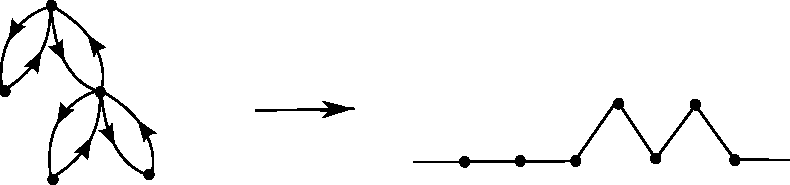
\includegraphics[width=1.00\textwidth]{Catalan-Pfad.pdf}
	\caption{Doppelbaum auf 5 Knoten und dem zugehörigen Catalan-Pfad} 
\end{figure}

%Lässt man die Wurzel außen vor, liegen \(r\ k\)-Knoten in den ungeraden Ebenen und \(l-r\ j\)-Knoten in den geraden Ebenen. Damit ergibt sich aus dieser Konstruktion, dass \(l-r\) die Anzahl der Aufstiege (und Abstiege) und \(2r\) die Anzahl der Flachstücke im Catalan-Pfad sind.  Denn: zu jedem \(j\)-Knoten führt genau eine Kante aus einer unteren Ebene hin und es führt genau eine Kante in eine untere Ebene zurück (Doppelbaum!). \\
Die Abbildung von den Doppelbäumen auf die Catalanpfade ist eine Bijektion, da:
\begin{itemize}
 \item[•]Da der Graph eulersch ist, ist $ \sum_{i=1}^{2l} $ =0; Der Graph ist immer über 0, ansonsten würde es ein m geben, sodass $ \sum_{i=1}^{2m-1}s^{i}=-1, ~\sum_{i=1}^{2m}s^{i}=0, ~ s_{2m-1}=-1  $. Also könnten wir einen Doppelbaum mit Knoten {1,2,...2m} konstruieren, und da $ s_{2m-1}=-1  $ ist, würde eine Kante von diesem Knoten zurück zu einem der ersten 2m Knoten gehen, was dem Aufbau eines Doppelbaums widersprechen würde. Insgesamt haben wir also einen Catalanpfad konstruiert. 
 \item[•] Surjektivität: Starte bei der Wurzel. Füge für jede Aufstiegskante einen Knoten in die nächst höhere Ebene und eine Kante als Verbindung hinzu. Füge für jede Abstiegskante eine Kante in die nächst niedriegere Ebene hinzu, bis die Doppelbaumstruktur vollständig ist. (Sollen wir das noch in Formeln übersetzen oder reicht das so?) 
%für jeden Catalanpfad der Länge l der Form $\lbrace s_{i} \rbrace$, $ i \leq 2l, i \in \NN $ kann ein Doppelbaum als Urbild wie folgt konstruiert werden: für i gerade: $s_{i}=-1 \rightarrow $ gehe von $j_{i/2}$abwärts, bei $s_{i}=0  $ aufwärts; für i ungerade bei $s_{i}=1 $ aufwärts, bei $s_{i}=0 $ abwärts.
\item[•] Injektivität analog zur Übung (bzw muss man das unbedingt nochmal zeigen?)\\
\end{itemize}
Die betrachteten Doppelbäume haben s.o. ein kombinatorisches Gewicht von 
	\begin{equation}
		\begin{pmatrix} N\\ l+1-r\end{pmatrix} (l+1-r)! \begin{pmatrix} M(N)\\r\end{pmatrix} r!
	\end{equation}
Für N hinreichend groß ist dies genähert \(N^{l+1-r}M(N)^r\). Damit folgt:
	\begin{equation}
		\frac {1}{N^{l+1}} N^{l+1-r}M(N)^r =~ \left( \dfrac{M(N)}{N}\right)^{r}\to \alpha^r
	\end{equation}
und damit:
	\begin{align*}
		\beta_l &:= \lim_{N\to\infty} \langle \overline{L_N}, x^l \rangle\\
		&= \lim_{N \to \infty} \sum_{J,K: v(J)+v(K) = l+1} \dfrac{1}{N^{l+1}}\EE[Y_N(J,K)]
		&= \sum_{r=1}^{l} \sum_{p_{r} \in C_{l}} \alpha^{r} = \sum_{p\in C_l} \alpha^r
	\end{align*}
wobei \(r=\#\{\text{Abstiege von ungeraden auf gerade Niveaus in } C_l\}\), und \(p_r\) Catalan-Pfad mit \(r\) entsprechenden Abstiegen.

Formel ist leider falsch. Wir brauchen die Formel aber anscheinend gar nicht.
%Ich denke, dass die Formel nun ist: 	
%	\[\beta_l = \sum_{r=1}^l \alpha^r\ \begin{pmatrix} l-1\\r-1\end{pmatrix} C_{l-r} \]
%und enstrechend für \(\gamma_l\) einfach die Einträge im Binomialkoeffizienten halbieren...Was meint ihr? Die Rechnung unten funktioniert dann weiterhin genauso! :)\\

%\(r = \frac 1 2 \#\{\text{Flachstücke in }C_l\} = l  - \#\{\text{Anstiege in }  C_l\}\), und $ p_{r} $ Catalanpfad mit 2r Flächenstücken.\\



%An Manu: kannst du diese Formel für \(\beta_l\) genauer erklären? Ich verstehe nicht wirklich, was du da machst...\\


%Mach ich. Also ich hab lang nicht verstanden, was das Kombinatorik-zeug vorne dran mit den Catalanpfaden zu tun hat. Du hattest glaub ich $C_l$ als Anzahl der Catalanpfade. Beim Überlegen für (10) dem nächsten Punkt hab ich mir dann die Formel für die Pfade gebaut, die im Grunde nur auf deiner Konstruktion basiert (und von der bist du ja hoffentlich überzeugt:) )\\
%$ \longrightarrow $Also wir brauchen die Anzahl der Catalanpfade, durch die wir unsere Doppelbäume beschreiben, weil's eine Bijektion ist. Nur haben wir andere Catalanpfade als die normalen:)\\
%Die Catalanpfade, die wir in der Vorlesung gebaut haben, mit der Anzahl $C_l$ (Catalanzahlen), sind dadurch definiert, dass du bei jedem Schritt + oder - 1 gehst, und das nichtüberkreuzend. \\ Bei unseren Catalanpfaden hast du aber noch deine "Flachstücke" mit 0 eingebaut! Und zwar 2r von denen. Also wie viele gibts von denen für ein bestimmtes r? Nach Konstruktion mit einem Knoten, sagen wir mal den j1, als Wurzel, sind der erste und letzte Schritt in dem Pfad auf jeden Fall flach, also 0. Da gibt's keine andere Möglichkeit. Von den restlichen 2l-2 Schritten im Pfad sind noch 2r-2 flach, die suchen wir als erstes raus. Das macht dann die $\begin{pmatrix} 2l-2\\2r-2\end{pmatrix} $.\\ 
%Bleiben uns noch 2l-2-(2r-2) Schritte übrig, die mit +/-1 zu belegen sind. Und zwar nichtüberkreuzend. Was das gleiche ist wie wenn du einen l-r-langen Catalanpfad bauen willst, weil du die 2r Flachstücke einfach mal ignorierst, die ändern ja nichts. Daher kommt das $ C_{l-r} $. Und wir haben die Anzahl!\\ Über r aufsummieren, damit wir alle Fälle mit r Knoten aus M(N), Rest aus N, haben. Das übrige Kombinatorik-zeug ist ja $\alpha^r  $, und schon steht die Formel da\\
%Die Formel für die Anzahl der Catlanpfade ist ganz praktisch für (10), für $ \beta$ selber brauchen wir sie ja erst mal nicht, deshalb wieder umcshreiben in $ \sum_{r} \alpha^{r} \#\{ \text{Catalanpfade mit 2r Flachstücke} \}$. Wenn du sie mal die Anzahl nimmst, kannst auch über alle 2r-Catalanpfade aufsummieren, das hoch r ändert sich ja nicht. Und dann $= \sum_{r=1}^{l} \sum_{p_{r} \in C_{l}} \alpha^{r} = \sum_{p\in C_l} \alpha^r $.\\ \\
%kurze Erklärung der Schritte schreib ich auch noch irgendwann oben rein.\\
% -> Danke für die Erklärung, davon sollten wir einiges in die spätere Endfassung ausfnehmen, damit die Formeln klarer werden! Was ich vllt hätte hinschreiben sollen ist, dass es bei mir beim vorletzten = hakt, also da, wo du die \(p_r\) einführst... \\ Jetzt mit richtiger Defintion von $ p_r $ klarer? \\

%\textbf{Beweis von  $\beta_{l}= \alpha \gamma_{l}$:}
Mit \(\beta_0 :=1, \gamma_0:=1 \) und
\begin{equation*}
		\gamma_l:=\sum_{p\in C_l} \alpha^{l-r} \qquad (l\geq 1)
\end{equation*}
gelten die Relationen
\begin{equation}
	\beta_l = \alpha\gamma_l=\alpha\sum_{r=0}^{l-1}\beta_r \gamma_{l-1-r}
\end{equation}
für alle \(l\geq 1\):\\
(\(l-r\) ist dabei die Anzahl der Abstiegskanten von geraden auf ungerade Niveaus im Catalan-Pfad.)
\begin{itemize}
%	\item \begin{equation}
%	\begin{split}
%\alpha \gamma_{l} =& \sum_{p \in C_l} \alpha^{l+1-r},\\
%\beta_l - \alpha \gamma_l =& \sum_{r=1}^{l} \alpha^r\ \begin{pmatrix} 2l-2\\2r-2\end{pmatrix} C_{l-r} - \sum_{r=1}^{l} \alpha^{l+1-r}\ \begin{pmatrix} 2l-2\\2l-2r\end{pmatrix} C_{r-1}   \\ 
%\underset{\text{Symmetrie Binom.}}{=}& \sum_{r=1}^{l} \begin{pmatrix} 2l-2\\2l-2r\end{pmatrix} \left( C_{l-r} \alpha^r - C_{r-1}\alpha^{l+1-r} \right) \\
%\overset{!}{=}& 0 \\
%\end{split}
%\end{equation}
%Für die einzelnen Summenglieder folgt:
%\begin{align*}
%\text{i-tes Summenglied:} &\begin{pmatrix} 2l-2\\2l-2i\end{pmatrix} \left( C_{l-i} \alpha^i - C_{i-1}\alpha^{l+1-i} \right) \\
%\text{(l+1-i)-tes Summenglied:}& \begin{pmatrix} 2l-2\\2l-2-2l+2i\end{pmatrix} \left( C_{l-1-l+i} \alpha^{l+1-i} - C_{1+l-i-1}\alpha^{l+1-1-l+i} \right)\\
% &= - \text{i-tes Summenglied}  
%\end{align*}
%Ist l gerade, dann heben sich folglich alle Summenglieder weg und die Summe ist 0, ist l ungerade, bleibt nur das (l+1)/2-te Summenglied übrig:
%\begin{align*}
% &\begin{pmatrix} 2l-2\\l+1-2\end{pmatrix} \left( C_{l-\frac{l+1}{2}} \alpha^{\frac{l+1}{2}} - C_{\frac{l+1}{2} -1}\alpha^{l+1-\frac{l+1}{2}} \right)\\
%&=\begin{pmatrix} 2l-2\\l-1\end{pmatrix} \left( C_{\frac{l-1}{2}} \alpha^{\frac{l+1}{2}} - C_{\frac{l-1}{2}}\alpha^{\frac{l+1}{2}} \right)=0
%\end{align*}

%Damit gilt der erste Teil von \((2.10)\)\\
\item
Betrachte die Position im Pfad, an der zum ersten Mal die \(0\) erreicht wird. Diese ist immer gerade, da die \(0\) genau dann erreicht wird, wenn man im zugehörigen Doppelbaum zur Wurzel zurückkehrt. Sei also \(2j\), \(j\in\{1,...,l\}\), diese Position. \\
Teile nun den Pfad in einen vorderen Teil \(P_1\) der Länge \(2j\) und einen hinteren Teil \(P_2\) der Länge \(2l-2j\). In dem erzeugenden Baum entspricht \(P_1\) dem äußersten Teilbaum, \(P_2\) dem restlichen Baum. \(P_2\) ist also ein beliebeiger Catalan-Pfad. \(P_1\) hat die besondere Struktur, dass die \(0\) erst an letzter Position erreicht wird, die erste und letzte Kante sind somit als Auftsiegs- bzw. Abstiegskante festgelegt und können für die kombinatorische Analyse vernächlässigt werden. Löscht man diese beiden Kanten und subtrahiert \(1\) von allen Elementen von \(P_1\), erhält man einen neuen Pfad \(\tilde{P}_1\), der ein beliebiger Catalan-Pfad der Länge \(2j-2\) ist. Dies folgt direkt aus der Struktur des Doppelbaumes: \(\tilde{P}_1\) entspricht dem äußersten Teilbaum ohne die ursprüngliche Wurzel, wodurch man einen neuen, beliebigen Doppelbaum erhält. \\
Die geraden/ungeraden Niveaus im ursprünglichen Pfad sind in \(\tilde{P}_1\) ungerade/gerade (Durch die Verschiebung um \(1\) nach unten). \(r\) und \(l-r\) haben sich also genau vertauscht!
\begin{figure}[htpb]
	\centering
	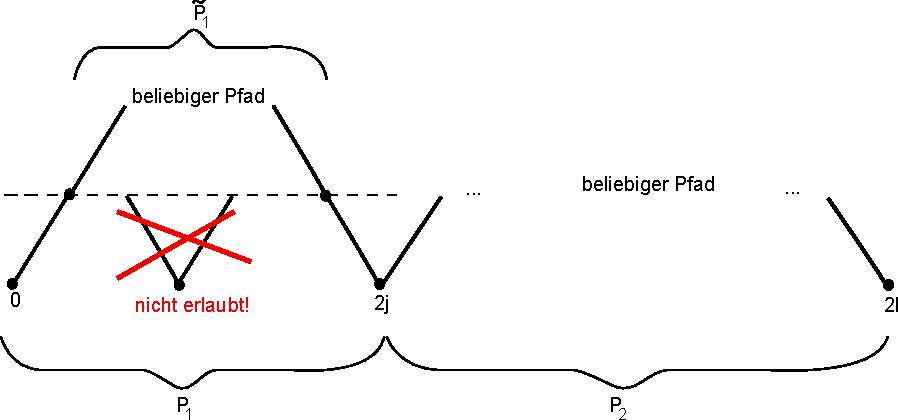
\includegraphics[width=1.00\textwidth]{Rekursion-Visualisierung.pdf}
	\caption{Schematische Darstellung der Rekursion}
\end{figure}
Damit ergibt sich aus den Definition für \(\beta_l\) und \(\gamma_l\) die Formel:
\begin{equation}
	\begin{split}
		\beta_l &= \alpha\sum_{j=1}^{l-1}\gamma_{j-1}\beta_{l-j} = \alpha\sum_{j=0}^l \gamma_j\beta_{l-j-1}\\
		&=\alpha\sum_{k=0}^l \beta_k\gamma_{l-1-k}
	\end{split}
\end{equation}
Das zusätzliche \(\alpha\) wird in der Formel durch das Löschen der Abwärtskante in \(P_1\) hervorgerufen.\\


\item $ \gamma $ wird analog rekursiv dargestellt: Im Gegensatz zu vorher tragen nun die Abwärtskanten von gerade zu ungerade zum Gewicht von $ \alpha $ bei. Sei wieder \(2j\), \(j\in\{1,...,l\}\), die Position, an der zum ersten Mal die \(0\) erreicht wird.. \\
Teile wiederum den Pfad in einen vorderen Teil \(P_1\) der Länge \(2j\) und einen hinteren beliebigen Catalanpfad \(P_2\) der Länge \(2l-2j\). In \(P_1\) sind wieder die erste und letzte Kante festgelegt. Beim Löschen dieser Kante werden die Ebenen vertauscht. \\
Anders als bei den $ \beta_l $ haben wir durch das Löschen der Abwärtskante allerdings kein $ \alpha $ verloren, da nun ja die Abwärtskanten von gerade zu ungerade das Gewicht $ \alpha $ haben.\\ 
Damit gilt: 
\begin{equation}
	\begin{split}
		\gamma_l &=\sum_{k=0}^l \beta_k\gamma_{l-1-k} \\
		&= \dfrac{\beta_l}{\alpha}
	\end{split}
\end{equation}

%Die Konstruktion der Catalan-Pfade aus der Doppelbaumstruktur ermöglicht eine weitere Interpretation von \(r\) bzw. \(l-r\):\\
%\begin{align*}
%	r&=\# \{\text{Schritte von gerader Ebene zu \underline{höherer} ungerader Ebene}\} \\
%	l-r &= \#\{\text{Schritte von ungerader Ebene zu \underline{höherer} gerader Ebene}\}
%\end{align*}
%Seien dies die \(r\)- bzw. \(l-r\)-Kanten, die im zugehörigen Catalan-Pfad an ungerader bzw. gerader Position liegen.\\
%Aus der Konstruktion der Catalan-Pfade aus der Doppelbaum-Struktur ergibt sich, dass das erste und letzte Element immer Flachstücke sind. Habe ein solcher Pfad der Länge l die Bezeichnung \(\tilde{C}_l\). Für so ein \(\tilde{C}_l\) gilt, dass die \(0\) zum ersten Mal (abgesehen von dem beginnenden Flachstück) nach einer ungeraden Anzahl von Schritten erreicht wird. Auf \(0\) kommt der Pfad nämlich immer nach erreichen eines Knotens in der ersten Ebene des erzeugenden Baumes, was nur nach einer ungeraden Anzahl von Kantendurchläufen möglich ist. Sei \(2j+1\) diese Position.\\
%Teile \(\tilde{C}_l\) in zwei Teilpfade wie folgt (für \(j>0\)):\\
%Sei \(P_1\) der Pfad von Position \(1\) bis \(2j+1\) und \(P_2\) der zusammengesetzte Pfad von Position \(0\) bis \(1\) und von \(2j+2\) bis \(2l\).\\
% \(P_2\) hat also Länge \(2l-2j\) und hat die Eigenschaft, dass das erste und letzte Element Flachstücke sind, \(P_2\) ist also von der Form \(\tilde{C}_{l-j}\). \(P_1\) hat Länge \(2j\), wobei das erste und letzte Element als auf- bzw. absteigende Kante festgelegt sind, da die \(0\) erst an letzter Position erreicht werden soll. Löscht man nun diese beiden Kanten, hat \(P_1\) noch Länge \(2j-2\) und ist von der Form \(\tilde{C}_{j-1}\), da (falls \(j>1\)) nach einer aufsteigenden Kante stets ein Flachstück und vor einer absteigenden Kante ebenfalls stets ein Flachstück liegt. (vgl. Konstruktion). Habe dieser Pfad den Namen \(\tilde{P}_1\).\\
%Die Kanten, die in \(P_1\) an gerader/ungerader Postion lagen, liegen auch in \(\tilde{P}_1\) an gerader/ungerader Positon, wohingegen sich bei \(P_2\) diese Eigenschaft genau umgekehrt hat, die \(r\)- und \(l-r\)-Kanten haben ihre Positionen vertauscht. Aus der Definiton von \(\beta_l\) und \(\gamma_l\) ergibt sich somit die rekursive Formel 
%\begin{equation}
%	\beta_l =\alpha\sum_{j=1}^l \beta_{j-1}\gamma_{l-j}=\alpha\sum_{j=0}^{l-1}\beta_j\gamma_{l-1-j}
%\end{equation}
%Das zusätzliche \(\alpha\) wird durch das Löschen der Aufwärtskante bei der Konstruktion von \(\tilde{P}_1\) hervorgerufen.

\end{itemize}
\textbf{Beweis von Formel (12)}\\
\begin{align*}
	Q_n :=& \alpha^{-1-n/2}\int_{\RR} f_{\alpha}(x)x(x-\alpha -1)^n\,\mathrm{d}x \\
	 =& \frac{1}{2\pi}\alpha^{-1-n/2} \int_{(1-\sqrt{\alpha})^2}^{(1+\sqrt{\alpha})^2} \sqrt{(x-(1-\sqrt{\alpha})^2)((1+\sqrt{\alpha})^2-x)} (x-\alpha -1)^n \,\mathrm{d}x\\
	=& \frac{1}{2\pi}\alpha^{-1-n/2} \int_{(1-\sqrt{\alpha})^2}^{(1+\sqrt{\alpha})^2} \sqrt{-\alpha^2+2\alpha x+2\alpha -x^2+2x-1}(x-\alpha-1)^n \,\mathrm{d}x\\
	\overset{x=y+\alpha+1}{=}& \frac{1}{2\pi}\alpha^{-1-n/2} \int_{-2\sqrt{\alpha}}^{2\sqrt{\alpha}} \sqrt{4\alpha -y^2} y^n \,\mathrm{d}y\\
	\overset{y=2\sqrt{\alpha}z}{=}& \frac{1}{2\pi}\alpha^{-1-n/2} \cdot 2^n \alpha^{n/2}\cdot4\sqrt{\alpha}\int_{-1}^{1} \sqrt{1-z^2}z^n \,\mathrm{d}z = \frac{2}{\pi} \cdot 2^n\int_{-1}^{1} \sqrt{1-z^2}z^n\,\mathrm{d}z \\
	\overset{\text{Übung 1}}{=}& \sigma(z^n) = \begin{cases} 0, &n\text{ ungerade}\\
	C_{\frac n 2}, &n\text{gerade} \end{cases}
\end{align*}
(Falls wir noch Platz füllen müssen, können wir hier die Rechnung aus der Übung auch wiederholen ;) )
Bei den "`Verständnis-Fragen"' habe ich jedoch etwas Probleme: \(f_{\alpha}\) ist für x=0 gar nicht definiert? Durch die Rechnung ergibt sich aber der Bezug zu \(\sigma(x)\), wo man dann doch beim Halbkreisgesetz wäre.\\
Zur Eindeutigkeit von \(f_{\alpha}\) sind diese "`verallgemeinerten Momente"' ein Problem. Habt ihr in der großen W-Theorie Vorlesung dazu was gemacht?\\


Ann: Theorem der Vorlesung auch für verallgemeinerte Momente anwendbar: f eind. bestimmt wenn $ Q_n< \infty $ (folgt aus (12)) und $ \sum_{n=0}^{\infty} Q_n \dfrac{z^n}{n!}$ positiven Konvergenzradius besitzt.\\
\[ \sum_{n=0}^{\infty} Q_n \dfrac{z^n}{n!}= \sum_{n=0}^{\infty} a_n z^n\]\\
wobei \[ a_n=\begin{cases} 0, &n\text{ ungerade}\\
	\dfrac{C_{\frac n 2}}{n!}=((\frac{k}{2}+1)!\frac{k}{2}!)^{-1}, &n\text{ gerade} \end{cases} \]
	Wurzelkriterium für Konvergenzradius: 
	\[(\frac{k}{2}+1)!\frac{k}{2}! \geq 1 \Rightarrow \vert a_n \vert \leq 1 \Rightarrow \]
	\[ r=(\limsup_{n \to \infty} \sqrt[n]{\vert a_n} \vert )^{-1} >1 \]
	


\textbf{Beweis von Formel (14)}\\
\begin{equation}
R_n=\lim_{N \to \infty} \alpha^{-1-n/2} \int_{\RR}\overline{L_{N}}(dx)x(x-\alpha-1)^{n} 
\end{equation}
Anwendung des binomischen Lehrsatzes ergibt:
\begin{align*}
 R_n =& \alpha^{-1-n/2} \lim_{N \to \infty} \int_{\RR}\overline{L_{N}}(dx)x \sum_{k=0}^n \begin{pmatrix} n\\k\end{pmatrix} x^{n-k}(-\alpha -1)^k \\
 =& \alpha^{-1-n/2} \lim_{N \to \infty} \langle \overline{L_{N}}, \sum_{k=0}^n \begin{pmatrix} n\\k\end{pmatrix} x^{n+1-k}(-\alpha -1)^k \rangle \\
 =& \alpha^{-1-n/2}\sum_{k=0}^n \begin{pmatrix} n\\k\end{pmatrix} (-\alpha -1)^k \beta_{n+1-k}
\end{align*}

wegen $\beta_l = \lim_{N\to\infty} \langle \overline{L_N}, x^l \rangle$ und der Linearität des Integrals.\\

Um die Rekursionsformel zu zeigen benötigt man folgende Formel:
\begin{equation}
	\sum_{n \geq t} \binom{m-n}{m-u-t} \binom{n}{t} = \binom{m+1}{u}
\end{equation}
Dies kann man kombinatorisch begründen. Stellt man sich das Pascalsche Dreieck vor, so gibt t die Diagonale und der Index n die Zeile vor. Der Binomialkoeffizient \(\binom{m+1}{u}\) ist die Anzahl der Pfade im Baumdiagramm...Fortsetzung folgt. \\

Nun betrachtet man:
\begin{align*}
\sum_{n=0}^m R_{m-n} R_n 
&= \sum_{n=0}^m \sum_{k=0}^{m-n} \binom{m-n}{k} (-\alpha -1)^k \beta_{m-n+1-k} \alpha^{-1-\frac{m-n}{2}} \sum_{l=0}^n \binom{n}{l} (-\alpha -1)^l \beta_{n+1-l} \alpha^{-1-\frac{n}{2}} \\
&= \alpha^{-1-\frac{m}{2}} \sum_{n=0}^m \sum_{l=0}^n \sum_{k=0}^{m-n} \binom{m-n}{k}  \binom{n}{l} (-\alpha -1)^{k+l} \beta_{m-n+1-k} \gamma_{n+1-l}	
\end{align*}

Der Index $k$ kann man durch $u:=k+l$ ersetzen.

\[\sum_{n=0}^m R_{m-n} R_m = \alpha^{-1-\frac{m}{2}} \sum_{n=0}^m \sum_{l=0}^n \sum_{u=l}^{m+l-n} \binom{m-n}{u-l}  \binom{n}{l} (-\alpha -1)^u \beta_{m-n+1+l-u} \gamma_{n+1-l}\]

Mit $t:=n-l$ kann $l$ umgeschrieben werden.

\begin{align*}
\sum_{n=0}^m R_{m-n} R_n 
&= \alpha^{-1-\frac{m}{2}} \sum_{n=0}^m \sum_{t=0}^n \sum_{u=n-t}^{m-t} \binom{m-n}{u-n+t}  \binom{n}{t} (-\alpha -1)^u \beta_{m+1-u-t} \gamma_{1+t} \\
&= \alpha^{-1-\frac{m}{2}} \sum_{t=0}^m \sum_{u=0}^{m-t} \sum_{n=t}^{u+t} \binom{m-n}{u-n+t}  \binom{n}{t} (-\alpha -1)^u \beta_{m+1-u-t} \gamma_{1+t} \\
&= \alpha^{-1-\frac{m}{2}} \sum_{t=0}^{m} \sum_{u=0}^{m-t} (-\alpha -1)^u \beta_{m+1-u-t} \gamma_{1+t} \sum_{n=t}^{u+t} \binom{m-n}{m-u-t}  \binom{n}{t}
\end{align*}

Mit Formel (2.14) gilt schließlich:

\begin{align*}
\sum_{n=0}^m R_{m-n} R_n 
&= \alpha^{-1-\frac{m}{2}} \sum_{t=0}^m \sum_{u=0}^{m-t} (-\alpha -1)^u \beta_{m+1-u-t} \gamma_{1+t} \binom{m+1}{u} \\
&= \alpha^{-1-\frac{m}{2}} \sum_{u=0}^{m+1} \binom{m+1}{u} (-\alpha -1)^u \sum_{t=0}^{m-u} \beta_{m+1-u-t} \gamma_{1+t}
\end{align*}

Durch die Substitution $r := m+1-u-t$ und die Anwendung von Formel (10) ergibt sich folgendes:

\begin{align*}
\sum_{n=0}^m R_{m-n} R_n
&= \alpha^{-1-\frac{m}{2}} \sum_{u=0}^{m+1} \binom{m+1}{u} (-\alpha -1)^u \left( \sum_{r=0}^{m+1-u} \beta_r \gamma_{m+2-u-r} - \beta_0 \gamma_{m+2-u} \right) \\
&= \alpha^{-1-\frac{m}{2}} \sum_{u=0}^{m+1} \binom{m+1}{u} (-\alpha -1)^u \left( - \beta_{m+2-u} + \sum_{r=0}^{m+2-u} \beta_r \gamma_{m+2-u-r} - \alpha^{-1} \beta_{m+2-u}\right) \\
&= \alpha^{-1-\frac{m}{2}} \sum_{u=0}^{m+1} \binom{m+1}{u} (-\alpha -1)^u \left(\frac{1}{\alpha} \beta_{m+3-u} - \dfrac{\alpha +1}{\alpha}\beta_{m+2-u} \right) \\
&= \alpha^{-1-\frac{m}{2}} \sum_{u=0}^{m+2} \binom{m+1}{u} (-\alpha -1)^u \frac{1}{\alpha} \beta_{m+3-u} \\
&- \alpha^{-1-\frac{m}{2}} \sum_{u=0}^{m+1} \binom{m+1}{u} (-\alpha -1)^u \dfrac{\alpha +1}{\alpha}\beta_{m+2-u} \\
&= \alpha^{-1-\frac{m}{2}} \sum_{u=0}^{m+2} \left( \binom{m+2}{u} -\binom{m+1}{u-1} \right) (-\alpha -1)^u \frac{1}{\alpha} \beta_{m+3-u} \\
&- \alpha^{-1-\frac{m}{2}} \sum_{u=0}^{m+1} \binom{m+1}{u} (-\alpha -1)^u \dfrac{\alpha +1}{\alpha}\beta_{m+2-u} \\
\end{align*}

(...)\\






{$ R_m=Q_m $:}\\
Dazu zeigen wir, dass $ R_0=Q_0 $ und $ R_1=Q_1 $, sowie dass die weiteren Folgenglieder von $ Q_m $ durch die gleiche Rekursionsformel gebildet werden können. Daraus folgt $ R_m=Q_m ~ \forall m$ \\

Beweis: \begin{align*}
\beta_1=& \alpha \beta_0 \gamma_0 = \alpha \\
\beta_2=& \alpha \beta_0 \gamma_1 + \alpha \beta_1 \gamma_0 = \alpha \gamma_1 + \alpha \beta_1 = \beta_1 + \alpha \beta_1  \\
R_0 =& \lim_{N \to \infty} \alpha^{-1} \int_{\RR}\overline{L_{N}}(dx)x = \dfrac{\beta_1}{\alpha}=1 \\
R_1 =& \alpha^{\frac{3}{2}} \lim_{N \to \infty}\int_{\RR}\overline{L_{N}}(dx)(x^2 - (\alpha +1)x)= \alpha^{\frac{3}{2}} (\beta_2 - (\alpha+1)\beta_1)=0 \\
Q_0=& C_0 =1, ~~Q_1=0
\end{align*}
Rekursion für $ Q_m: $

\begin{align*}
\text{m ungerade:}& \sum_{n=0}^m Q_{m-n}Q_n= Q_0 \underbrace{Q_m}_{\substack{=0}} + \underbrace{Q_1}_{\substack{=0}}Q_{n-1}+....= 0=Q_{m+2}\\
\text {m gerade:}&~ Q_{m+2}= C_{\frac{m}{2}+1}= \sum_{k=0}^{\frac{m}{2}} C_k C_{\frac{m}{2}-k}=\sum_{k=0}^{\frac{m}{2}} Q_{2k}Q_{m-2k}=\sum_{n=0}^{m}Q_n Q_{m-n}
\end{align*}
wobei der letzte Schritt aus $ Q_n Q_{m-n}=0 $ für $ n=2k+1 $ folgt.\\

Mit folgendem Theorem aus der Vorlesung kann die Aussage nun bewiesen werden.

\begin{theorem}
Sei \((\mu_n)_{n \in \NN}\) eine Folge in $\mathcal{M}(\RR)$ mit endlichen Momenten und $\mu \in \mathcal{M}(\RR)$ eindeutig durch seine Momente bestimmt. Dann gilt:
\[\forall l \in \NN_0: m_l(\mu) \rightarrow m_l(\mu) \Rightarrow \mu_n \overset{W}{\rightarrow} \mu\]
\end{theorem}

Für $l \geq 1$ existieren $\lambda_0,...,\lambda_{l-1} \in \RR$, sodass $x^l = \sum_{n=0}^{l-1} \lambda_n x (x-\alpha-1)^n$. Daraus folgt:
\begin{align*}
\forall l \in \NN: \lim_{N \to \infty} m_l(\overline{L_{N}}) 
&= \lim_{N \to \infty} \int_\RR x^l \overline{L_{N}}(dx)
= \lim_{N \to \infty} \int_\RR \sum_{n=0}^{l-1} \lambda_n x (x-\alpha-1)^n \overline{L_{N}}(dx) \\
&= \sum_{n=0}^{l-1} \lambda_n \lim_{N \to \infty} \int_\RR x (x-\alpha-1)^n \overline{L_{N}}(dx) \\
&= \sum_{n=0}^{l-1} \lambda_n R_n
= \sum_{n=0}^{l-1} \lambda_n Q_n = m_l(f_\alpha)
\end{align*}

Für den Fall l = 0 erhalten wir:
\[\lim_{N \to \infty} m_0(\overline{L_{N}}) 
= \lim_{N \to \infty} \int_\RR \overline{L_{N}}(dx) = 1 
= \int_\RR f_\alpha(x)dx\]

Um zu zeigen, dass $f_\alpha(x)dx \in \mathcal{M}(\RR)$ eindeutig durch seine Momente bestimmt ist, betrachtet man folgende Potenzreihe:

\[\sum_{l=0}^\infty m_l(f_\alpha) \frac{z^l}{l!}\]

$m_l(f_\alpha)$ auszurechnen ist wahrscheinlich auch nicht so einfach.

Bleibt zu zeigen, dass damit $ \overline{L_N} \overset{w}{\rightarrow} f_\alpha (x)dx~(N \rightarrow \infty) $. \\
Unter der Annahme, dass diese seltsamen "verallgemeinerten Momente" genauso wie die normalen Momente verwendet werden können, können wir das Theorem aus der Vorlesung anwenden, um von der Konvergenz der Momente auf die schwache Konvergenz der W-maße zu kommen. \\
Voraussetzungen: 1. $ f_\alpha $ ist durch $ Q_n $ eindeutig bestimmt, s.o. erfüllt;\\
2. \[ \alpha^{-1-n/2} \int_{\RR}\overline{L_{N}}(dx)x(x-\alpha-1)^{n} = \alpha^{-1-n/2}\sum_{k=0}^n \begin{pmatrix} n\\k\end{pmatrix} (-\alpha -1)^k \langle \overline{L_N}, x^{n+1-k} \rangle \] 
\[= \alpha^{-1-n/2}\sum_{k=0}^n \begin{pmatrix} n\\k\end{pmatrix} (-\alpha -1)^k \EE [\dfrac{1}{N} tr(W_N^{n+1-k})]
< \infty ~\forall N,n \in \NN_0 \]\\
wegen $ \sup_{j,k,N} \EE[\vert Y_N(j,k)\vert ^{q}]< \infty$ \\
(...okay sicher bin ich mir bei dem Ganzen nicht aber das hier ist alles mehr so als Idee aufzufassen)\\
$ \Rightarrow $ Theorem (Woche 2, Seite 3 rechts) $ \Rightarrow $ schwache Konvergenz




\end{document}
